
\documentclass[template=tabling,81pt,headonall]{azmoon}
\usepackage{xepersian}
\usepackage{amsfonts}
\usepackage{graphicx}
\usepackage{svg}
\svgpath{ {./images/} }
\graphicspath{ {./images/} }
\settextfont{Yas}
\setdigitfont{A Iranian Sans}
\usepackage{fontawesome5}

\printanswers
    \teacher{محمد صالح علی اکبری}
    \teachertitle{دبیر}
    \city{گناباد}
    \schooltitle{متوسطه دوره اول}
    \school{مقداد}
    \grade{نهم}
    \branch{۱}
    \topic{ریاضی}
    \examdate{دی ۱۴۰۲}
    \answertime{۹۰ دقیقه}
    \begin{document}
	\begin{questions}
		\nointerlineskip%
		\vskip-\baselineskip
		\question[1]{%
هر یک از مجموعه‌های زیر چند عضو دارند؟
    \begin{parts}[2]\part{\{۴ ، ۵، ۸\}}
\part{$\{\dfrac{4}{2} , \dfrac{6}{3}, 2\}$}
\end{parts}

    }\question[2]{%
مجموعه $S=\{1,2,3,4,5,6,7,8\}$ به این صورت است. برای هر یک از زیر مجموعه‌های این مجموعه که در زیر آمده مانند نمونه یک جمله نظیر کنید.
    \begin{parts}[2]\part{$A=\{8 , 7\}$ مجموعه تمام اعداد عضو S که در تاس وجود ندارند.}
\part{$B=\{2, 4, 6, 8\}$}
\part{$C=\{1 ,2 ,3 ,4 ,5 ,6\}$}
\end{parts}

    }\question[1]{%
حاصل عبارت‌های زیر را حساب کنید.
    \begin{LTR}
        \begin{parts}[2]\part{$ 200 - 100 + 30 = $}
\part{$5 -100 + 30 + 70 = $}
\end{parts}
\end{LTR}
        
    }\question[1]{%
حاصل عبارت‌های زیر را حساب کنید.
    \begin{LTR}
        \begin{parts}[2]\part{$-4 \times (-7) = $}
\part{$-16 \times (2) = $}
\part{$4 \times (-2)  = $}
\part{$5 \times (-6) = $}
\end{parts}
\end{LTR}
        
    }\question[2]{%
حاصل تقسیم‌های زیر را محاسبه کنید.
    \begin{parts}[4]\part{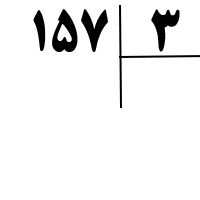
\includegraphics[scale = 0.18]{تقسیم3}}
\part{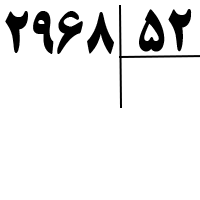
\includegraphics[scale = 0.18]{تقسیم9}}
\end{parts}
‌
\\‌
\\‌
\\
    }\question[2]{%
حاصل جمع و تفریق‌های زیر را محاسبه کنید.
    \begin{LTR}
        \begin{parts}[1]\part{$\dfrac{2}{3}+\dfrac{2}{7} = $}
\part{$\dfrac{1}{2}-\dfrac{3}{1} = $}
\part{$-\dfrac{4}{3}+\dfrac{1}{9} = $}
\end{parts}
\end{LTR}
        
    }\question[3]{%
حاصل ضرب و تقسیم‌های زیر را محاسبه کنید.
    \begin{LTR}
        \begin{parts}[1]\part{$+\dfrac{4}{5}\times \dfrac{3}{7} = $}
\part{$\dfrac{2}{3}\div\dfrac{4}{7} = $}
\part{$\dfrac{2}{3}\div\dfrac{7}{9} = $}
\end{parts}
\end{LTR}
        
    }\question[4]{%
حاصل عبارت‌های زیر را حساب کنید. \\ $\sqrt{2} \simeq 1.2 \sqrt{3} \simeq 1.7 \sqrt{5} \simeq 2.2  \sqrt{6} \simeq 2.4 \sqrt{7} \simeq 2.6 \sqrt{8} \simeq 2.8$
    \begin{LTR}
        \begin{parts}[1]\part{$|-3-2\sqrt{7}| = $}
\part{$|1-\sqrt{2}| = $}
\part{$|\sqrt{7} -\sqrt{2}| = $}
\part{$|\sqrt{4} -\sqrt{5}| = $}
\end{parts}
\end{LTR}
        
    }\question[2]{%
اگر امروز ۱۳ دی باشد و اسفندماه ۱۹ ۲۹ روزه باشد. چند روز تا ۱۵ مهر باقی مانده است؟}\question[2]{%
محیط و مساحت شکل زیر را محاسبه کنید. \\ 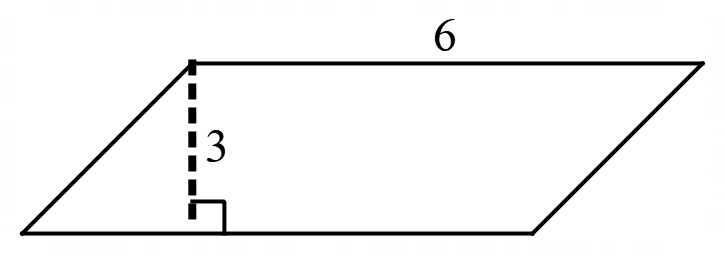
\includegraphics[scale = 1]{متوازی الاضلاع}}\end{questions}
    \end{document}
    